\section{TrustEpisode Reconstruction Contract}
\label{sec:method}

\trustepisode converts normalized EDR/NDR events and authenticated SourceCoverage into
version-scoped forensic audit records that are deterministic over canonicalized, version-bound
inputs. Episode Synthesis alone owns membership. The lifecycle is open episode $\rightarrow$
finalized revision $\rightarrow$ immutable late successor or closed lineage $\rightarrow$
beyond-horizon LateEvidenceRecord. Each revision yields exactly one terminal AssemblyOutcome
(a canonical AuditRecord or an immutable AssemblyFailureRecord). Analysts and AI systems consume
these records but cannot redefine membership, source health, probability support, or terminal status.
Optional Feature Extractor / Scorer / Scope Resolver / Calibrator fields and sufficiency $U$ remain
design-only schema interfaces. Figure~\ref{fig:method-architecture} shows these boundaries; ground
truth is joined only offline.

\subsection{Investigation and Threat Model}
\label{sec:threat-model}

\paragraph{Assumptions.}
Raw pointers and the sealed evidence store are integrity-checkable; Health Monitor coverage
messages have authenticated sources; attackers may induce missing events, delayed delivery, and
duplicate retries; attackers cannot arbitrarily forge signed health state; runtime software may
fault; the offline evaluator is isolated from online formation.

\paragraph{Non-assumptions.}
We do \emph{not} assume complete telemetry, that collector silence equals downtime, that all
attacks are observable, that ground truth is available online, that model scores are reliable, or
that raw arrival order is fixed. Compromise of the Health Monitor identity, signing keys, or an
external writer-authorization layer is outside scope; SHA-256 digests do not authenticate producers.

\paragraph{Downstream-agent adversary.}
An AI assistant may be mistaken, prompt-injected, or compromised: it may omit evidence, misquote a
record, or recommend an unsafe action. It is outside the trusted computing base and has no
capability to write canonical evidence objects. The contract does not make its narrative true; it
makes any cited case claim checkable against an immutable revision and prevents the narrative from
silently becoming the forensic record.

\paragraph{Investigator workflow.}
Investigators import sealed EDR/NDR, form revisions, and inspect each terminal audit outcome.
They then check coverage and provenance, resolve late evidence, run the A--G waterfall for a
missing step, replay the digests, and report observed, unavailable, and unknown separately.

\subsection{Evidence and Reconstruction Model}
\label{sec:problem-formulation}

The core evaluated objects are NormalizedEvent, SourceCoverage, EpisodeRevision,
LateEvidenceRecord, AuditRecord, and AssemblyFailureRecord; optional design-only schema objects
are FeatureVector, SupportDecision, nullable $P$, and structured $U$. Offline labels never enter
online schemas. Table~\ref{tab:ownership} assigns producers and forbidden behaviors for both.

\begin{table*}[!t]
\caption{Single-owner online object contract.}
\label{tab:ownership}
\centering
\scriptsize
\begin{tabular}{p{0.17\textwidth}p{0.17\textwidth}p{0.29\textwidth}p{0.28\textwidth}}
\toprule
\textbf{Object} & \textbf{Sole producer} & \textbf{Consumers} & \textbf{Forbidden behavior} \\
\midrule
NormalizedEvent & Evidence Fabric & Episode Synthesis & label, scenario, or health fields \\
SourceCoverage & Health Monitor & Scope Resolver; Sufficiency; Assembler & infer outage from event silence \\
EpisodeRevision / LateEvidenceRecord & Episode Synthesis & Feature; Sufficiency; Assembler / late store & rewrite a prior revision; admit beyond-horizon into membership \\
FeatureVector $[D,C]$ & Feature Extractor & Stateless Scorer; Assembler & health/source mask; labels; scenario metadata \\
Nullable $P$ & Calibrator (design) & Assembler & numeric unsupported output \\
Structured $U$ & Sufficiency Evaluator & Assembler & scalarization that rewrites $P$ \\
AssemblyOutcome & AuditRecord Assembler & Append-only store; replay & both success and failure; update/delete \\
\bottomrule
\end{tabular}
\end{table*}

\begin{figure}[t]
  \centering
  \scriptsize
  \setlength{\fboxsep}{5pt}
  \begin{minipage}{\columnwidth}\centering
  \fbox{\parbox{0.91\columnwidth}{\centering
    \textbf{EDR/NDR events + authenticated source health}}}\\[2pt]
  $\downarrow$\\[2pt]
  \fbox{\parbox{0.91\columnwidth}{\centering
    \textbf{Evidence Fabric / Health Monitor}}}\\[2pt]
  $\downarrow$\\[2pt]
  \fbox{\parbox{0.91\columnwidth}{\centering
    \textbf{Episode Synthesis (sole membership owner)}}}\\[2pt]
  $\downarrow$\\[2pt]
  \fbox{\parbox{0.91\columnwidth}{\centering
    \textbf{AuditRecord Assembler $\rightarrow$ append-only store}}}\\[2pt]
  \textit{Offline only: labels, matching, evaluation.}
  \end{minipage}
  \caption{Label-blind online reconstruction and offline evaluation boundary.}
  \Description{A four-stage vertical flow from EDR and NDR events plus source health, through
  Evidence Fabric and Health Monitor, Episode Synthesis, and AuditRecord assembly to an
  append-only store; labels and evaluation remain offline.}
  \label{fig:method-architecture}
\end{figure}

\subsection{Independent Evidence Health and Observability}
\label{sec:evidence-health}

Event silence is not an outage. ``No detection'' is not ``unavailable.'' SourceCoverage carries
authenticated health, parser validity, and an observed source mask. Assemblers consume exact
coverage references; they do not infer health from empty event windows.

\subsection{Deterministic Episode Formation}
\label{sec:episode-synthesis}

Formation links events using process-causal, authenticated-session, endpoint-connection, and
specific-entity relations under a 300\,s maximum inter-event gap and 3600\,s maximum episode
span. Tie-breaks are deterministic under the frozen canonical ordering contract (relation precedence,
relation count, $\Delta t$, start time, episode ID). Hub suppression, parent merge, and exact
event-time ordering are part of the frozen policy. Canonical event-time ordering is a mandatory
preprocessing step of the production formation path rather than an optional replay repair: raw
delivery order is not robust, whereas re-canonicalized input reproduces byte-identical results.
Formation never reads labels, receipts, or scenario metadata.

\begin{figure*}[t]
  \centering
  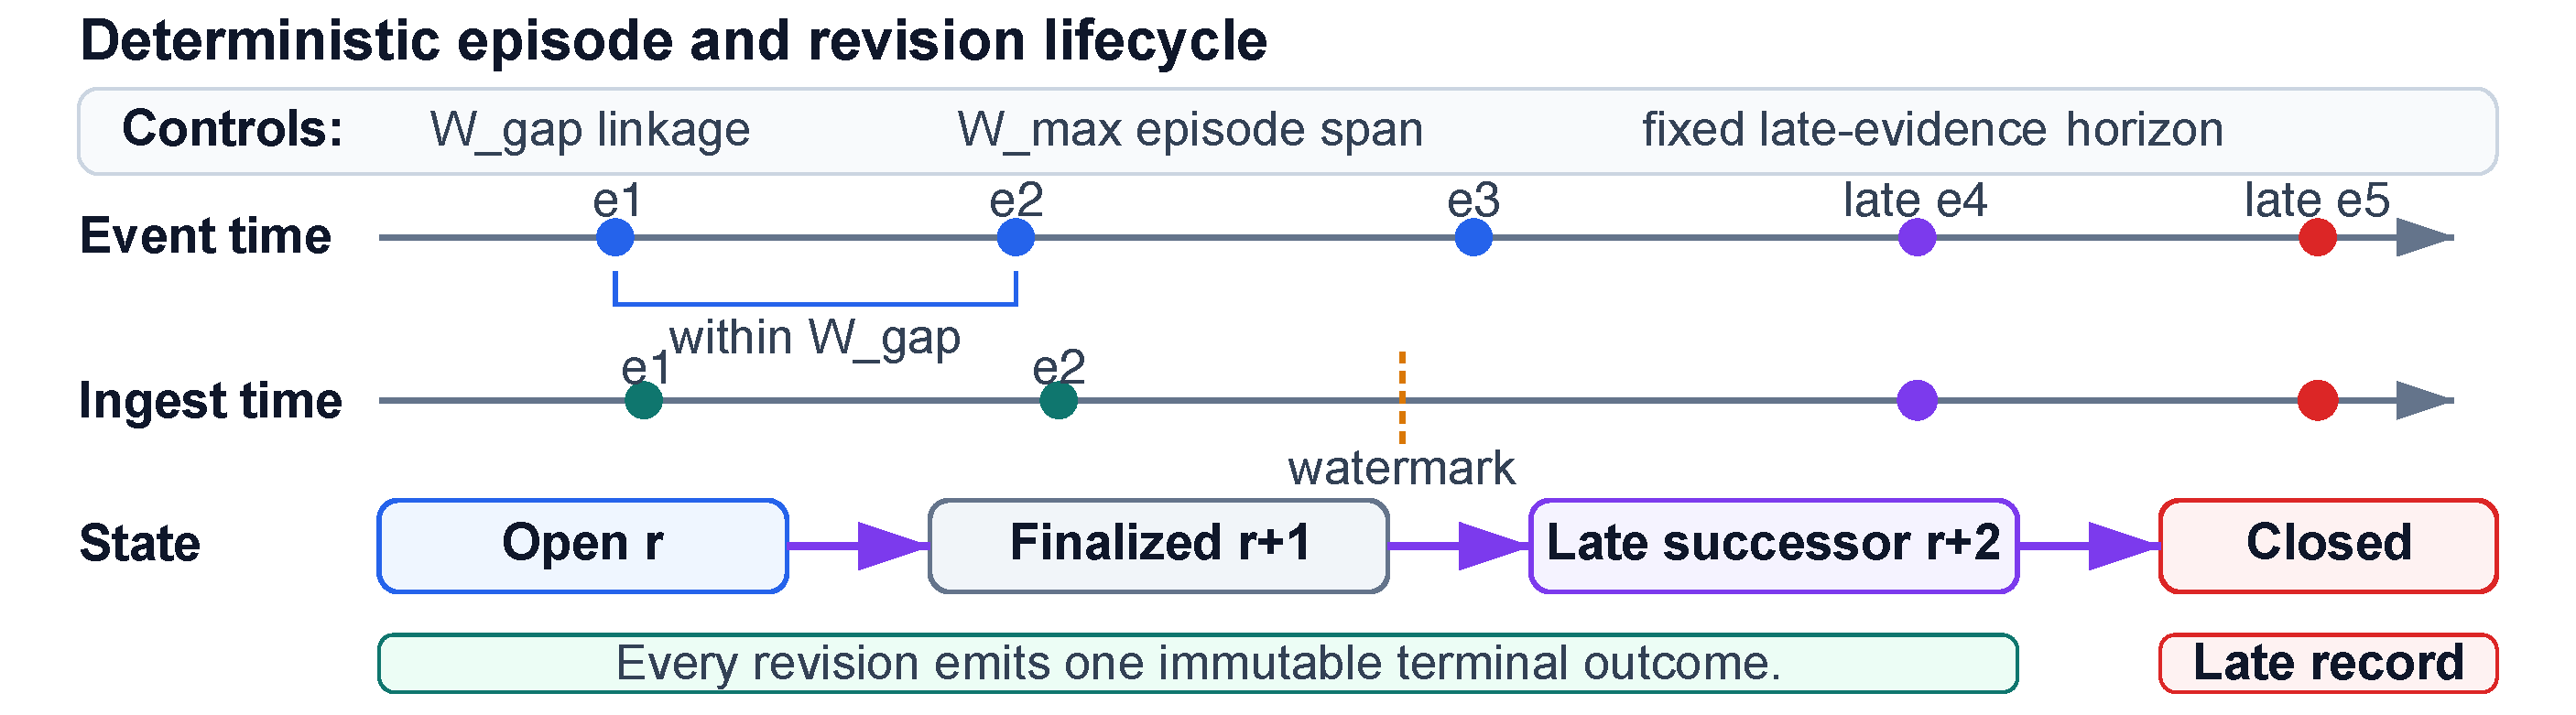
\includegraphics[width=\textwidth]{trustepisode_figures/pdf/fig02_episode_revision_lifecycle.pdf}
  \caption{Episode revision lifecycle: open $\rightarrow$ finalized $\rightarrow$ late successor or
  closed; beyond-horizon evidence enters LateEvidenceRecord without rewriting earlier membership.}
  \Description{A timeline showing event and ingest time, an open episode, finalization at a
  watermark, an immutable late-successor revision within the horizon, closure, and a separate
  late record beyond the horizon.}
  \label{fig:episode-revision-lifecycle}
\end{figure*}

\subsection{Immutable Revision Lifecycle}
\label{sec:revision-lifecycle}

A watermark lag of 120\,s advances the watermark behind observed ingest and finalizes open
episodes whose event-time end is at or before that watermark. Late evidence inside a fixed 900\,s
revision horizon may create an immutable successor; beyond-horizon or closed-lineage evidence
produces a LateEvidenceRecord. Earlier digests are never rewritten; deadlines are not extended by
late arrivals.

\subsection{Terminal Forensic Audit Contract}
\label{sec:audit-assembly}

Open episodes finalize once their event-time end is at or before the advancing watermark (lag
120\,s behind observed ingest). The assembler then applies a separate 120\,s join deadline
anchored at EpisodeRevision.watermark and inserts exactly one terminal outcome under
$(episode\_id,revision)$: AuditRecord or AssemblyFailureRecord (schema, key, duplicate, digest,
version, missing-input, timeout). These are distinct lifecycle deadlines with different anchors.
Success cannot follow terminal failure. References are canonically ordered; RFC~8785/JCS
serialization and SHA-256 digests bind versions. The store is append-only.

\subsection{Agent-Facing Evidence Boundary}
\label{sec:agent-boundary}

Downstream analyst views and AI assistants are consumers, never producers, of canonical case
facts. They receive a revision key, terminal AssemblyOutcome, ordered evidence references,
SourceCoverage references, and the independent sufficiency profile. A generated explanation or
recommended action is a noncanonical view: it cannot write EpisodeRevision, change $P$ or $U$, or
replace an AssemblyFailureRecord with success. If required inputs are missing, the only canonical
output is the failure record; an agent is not permitted to fill the gap from conversational
context. This boundary makes a later narrative falsifiable against immutable source references
without treating the language model as part of the forensic root of trust.
Section~\ref{sec:agent-boundary-conformance} tests closed-schema, support-coupling, provenance,
and digest guards. Section~\ref{sec:llm-grounding-pilot} then treats the model as an untrusted
reader and scores exact values, abstention, and pointer citations; service-identity authorization
remains a deployment assumption rather than an evaluated result.

\paragraph{Integrity is not writer authorization.}
The closed schema and unkeyed RFC~8785/SHA-256 digest validate object shape and detect an
unresealed change; they do not authenticate the producer. A downstream principal with canonical
write permission could change an allowed field and recompute the digest. The read-only boundary
therefore requires two layers: externally enforced writer authorization, plus the evaluated
schema/digest contract. AI7 is an expected-accept negative control that makes this dependency
explicit rather than treating a hash as a signature.

\subsection{Evidence-Loss Taxonomy}
\label{sec:evidence-loss-taxonomy}

When a required action token is absent from a reconstructed episode, diagnosis uses the following
closed classes (Table~\ref{tab:loss-taxonomy}):

\begin{table}[!t]
\caption{Evidence-loss taxonomy for incomplete reconstruction.}
\label{tab:loss-taxonomy}
\centering
\scriptsize
\setlength{\tabcolsep}{3pt}
\begin{tabular}{@{}>{\raggedright\arraybackslash}p{0.30\columnwidth}>{\raggedright\arraybackslash}p{0.62\columnwidth}@{}}
\toprule
\textbf{Class} & \textbf{Decision rule (summary)} \\
\midrule
\path{A_execution_failure} & Action receipt/predicate shows non-success \\
\path{B_sensor_observability_failure} & Receipt success but raw EDR/NDR lacks identifiable activity \\
\path{C_parser_or_normalization_failure} & Raw present; NormalizedEvent absent or rejected \\
\path{D_token_mapping_failure} & NormalizedEvent present under wrong/missing required token \\
\path{E_formation_membership_failure} & Correct token exists but not retained in matched episode \\
\path{F_offline_attribution_failure} & Episode retains evidence; matcher fails to credit token \\
\path{G_unknown_or_incomplete_trace} & Required supporting records missing for A--F \\
\bottomrule
\end{tabular}
\end{table}

Forbidden inference: treating episode-match F1~$=$~1.0 as exact-complete step recovery; treating
missing tokens as formation failures without a waterfall. In operational cases without a trusted
execution receipt or equivalent predicate record, the waterfall may terminate in G rather than
distinguishing execution failure from downstream evidence loss. Synthetic A--G fixtures exercise the
closed diagnostic taxonomy; they are not field validation.

\subsection{Scoring and Probability Extension (Design Only)}
\label{sec:calibration}

Design-only and unevaluated here: a Stateless Scorer consumes only $D$ and $C$ and emits
$z=f_{\theta}(D,C)$; a Scope Resolver separately consumes source availability / manifest scope and
emits a SupportDecision governing whether $P$ may be numeric. Source health must not influence $z$.
Without supported scope and a fitted version-matched calibrator, $P$ remains JSON null. Structured
$U$ cannot rewrite $z$ or $P$. This submission reports no fitted coefficients, Brier/NLL, or held-out
ranking.

\subsection{Boundary}
\label{sec:method-boundary}

The \emph{evaluated} contribution is deterministic reconstruction over canonicalized, version-bound
inputs and replayable audit semantics, including evidence-loss localization and a deployed read-only
case-materialization trace. Manifest-scoped probability is design-only. LLM generation quality, CTI
enrichment, impact scoring, autonomous response, and OT/ICS generalization are excluded.
